% \input{"IAB/latex/TeX-Folienformat.tex"}
\input{"/Users/jonathanlatner/Google Drive/My Drive/IAB/latex/TeX-Folienformat.tex"}

\documentclass[t,8pt,utfx8]{beamer}
\usepackage{booktabs}
\usepackage{setspace}
\usepackage{parskip}
\usepackage{graphicx}
\usepackage{subcaption}
\setbeamertemplate{caption}[numbered]
\newcommand{\sprache}{\englisch}
\renewcommand{\thesubsection}{\alph{subsection})}
\usepackage[cal=pxtx, scr=dutchcal]{mathalpha}


\usepackage{listings} %include R code

\definecolor{codegreen}{rgb}{0,0.6,0}
\definecolor{codegray}{rgb}{0.5,0.5,0.5}
\definecolor{codepurple}{rgb}{0.58,0,0.82}
\definecolor{backcolour}{rgb}{0.95,0.95,0.92}

\lstdefinestyle{mystyle}{
    backgroundcolor=\color{backcolour},   
    commentstyle=\color{codegreen},
    keywordstyle=\color{magenta},
    numberstyle=\tiny\color{codegray},
    stringstyle=\color{codepurple},
    basicstyle=\ttfamily\tiny,
    breakatwhitespace=false,         
    breaklines=true,                 
    captionpos=b,                    
    keepspaces=true,                 
    numbers=left,                    
    numbersep=5pt,                  
    showspaces=false,                
    showstringspaces=false,
    showtabs=false,                 
    columns=fullflexible,
    frame=single,
    tabsize=2
}

\lstset{style=mystyle}


\newcommand{\btVFill}{\vskip0pt plus 1filll}

\title{Generating synthetic data is complicated: Know your data and know your generator}
\subtitle{PSD2024: Privacy in Statistical Databases 2024, \newline 26. September, 2024}

\author{Jonathan Latner, PhD \newline Dr. Marcel Neunhoeffer \newline Prof. Dr. Jörg Drechsler}

\newcounter{noauthorlines}
\setcounter{noauthorlines}{2} % Wert für 2 Autoren über 2 Zeilen. Ggf. anpassen

% %%%%%%%%%%%%%%
% Ende Anpassung
% %%%%%%%%%%%%%%

% \input{"IAB/latex/TeX-Folienformatierung_CD_2019"}
\input{"/Users/jonathanlatner/Google Drive/My Drive/IAB/latex/TeX-Folienformatierung_CD_2019"}

% Modify the section in toc template to enumerate
\setbeamertemplate{section in toc}{%
    \inserttocsectionnumber.~\inserttocsection\par
}

% use for subsections
% \setbeamertemplate{subsection in toc}{}
\setbeamertemplate{subsection in toc}{%
    \setlength{\parskip}{1mm}
        \hskip2mm -- \hskip1mm\inserttocsubsection\par
}


\usepackage{colortbl}
\definecolor{lightgray}{gray}{0.9}


\begin{document}


\frame[plain]{\titlepage}

\begin{spacing}{1.25}

% %%%%%%%%%%%%%%
% Section
% %%%%%%%%%%%%%%

\section{Introduction}\label{sec:intro}
\frame{\frametitle{Section \ref{sec:intro}: Overview}

\begin{itemize}
    \item Common perception that making synthetic data is easy
    \item We want to show that its complicated
    \begin{itemize}
        \item You need to know your data
        \item You need to know your synthetic data generator (SDG)
        \item The problem: Individuals who know the data may not be the same as those who know the SDG
    % \item Contribution: While most research examining SDGs use `clean' data to evaluate SDGs, we use `real' data
    \end{itemize}
    \item Conclusion
    \begin{itemize}
        \item On the one hand, generating synthetic data is easy
        \item On the other hand, users need to be aware of challenges
        \item The point: One should be skeptical about automated, one-size-fits-all processes for generating synthetic data
    \end{itemize}
\end{itemize}
}

\frame{\frametitle{The good news -- making synthetic data is easy}

\begin{itemize}
    \item \url{Gretel.ai}: The synthetic data platform for developers. Generate artificial datasets with the same characteristics as real data, so you can develop and test AI models without compromising privacy.
    \item \url{Mostly.ai}: Synthetic Data. Better than real. Still struggling with real data? Use existing data for synthetic data generation. Synthetic data is more accessible, more flexible, and simply...smarter.
    \item \url{Statice.ai}: Generating synthetic data comes down to learning the joint probability distribution in an original, real dataset to generate a new dataset with the same distribution.  The more complex the real dataset, the more difficult it is to map dependencies correctly. Deep learning models such as generative adversarial networks (GAN) and variational autoencoders (VAE) are well suited for synthetic data generation.
    \item \url{hazy.com}: Synthetic data does not contain any real data points so can be shared freely. Say goodbye to lengthy governance processes associated with real data.  Specifically, Hazy data is designed to preserve all the patterns, statistical properties and correlations in the source data, so that it can be used as a drop-in replacement for it.
    \item DataSynthesizer (Ping et al., 2017): The distinguishing feature of DataSynthesizer is its usability — the data owner does not have to specify any parameters to start generating and sharing data safely and effectively.
\end{itemize}
}

\frame{\frametitle{The bad news -- making synthetic data is hard}

\begin{itemize}
    \item We must ask: 
    \begin{itemize}
        \item Why are we creating synthetic data?  (generating code, education, the public, etc.)
        \begin{itemize}
            \item How different should it be?  
            \item How do we measure the difference? 
        \end{itemize}
        \item How does the synthesizer work? 
        \begin{itemize}
            \item Variables types (categorical, continuous)
            \item Variable values (missing, extreme, and `spikey' values, etc.)
            \item How long it takes to generate synthetic data from original data (i.e. `computational efficiency')
        \end{itemize}
    \end{itemize}
    \item Answering these questions will help us make decisions about which synthesizer is the right choice
\end{itemize}
}



\frame{\frametitle{Our goal is to illustrate the challenges}
\begin{itemize}
    \item Know your data (1 dataset)
    \begin{itemize}
        \item Social Diagnosis 2011 (SD2011)
    \end{itemize}
    \item Know your generator
    \begin{itemize}
        \item Examine 3 synthetic data generators (SDGs): DataSynthesizer, CTGAN, Synthpop
    \end{itemize}
    \item 3 utility measures 
    \begin{itemize}
        \item Compare univariate frequency -- difference/similarity in one variable 
        \item Propensity score mean -- difference/similarity in the dataset (lower values better)
        \item Computationally efficiency -- duration in time required to generate synthetic data (lower values better)
    \end{itemize}
\end{itemize}
}

% %%%%%%%%%%%%%%
% Section
% %%%%%%%%%%%%%%

\section{Know your data}\label{sec:data}
\frame{\frametitle{Section \ref{sec:data}: Know your data (SD2011)}
\begin{itemize}
    \item Social Diagnosis 2011 (SD2011)
    \begin{itemize}
        \item Loads with Synthpop
        % \item \url{http://www.diagnoza.com/index-en.html}
        % \item Not entirely clear how original data is created or cleaned to create data in Synthpop
    \end{itemize}
    \item Like real data, has messy variables with unusual values
    \begin{itemize}
        \item Missing values
        % \begin{itemize}
        %     \item Informative (i.e. for never worked abroad, \texttt{wkabdur} is missing)
        %     \item Non-informative 
        % \end{itemize}
        \item `Errors'
        % \begin{itemize}
        %     \item \texttt{smoke} - Does smoke is NO, but \texttt{nociga} - 20/22 cigarettes per day 
        %     \item \texttt{bmi} = 451, but \texttt{height}(cm) = 149 and \texttt{weight}(kg) = NA (999)
        % \end{itemize}
        \item Generated variables (Can be problematic for SDGs)
        % \begin{itemize}
        %     \item \texttt{bmi,agegr}
        % \end{itemize}
        \item `Spikey' or discontinuous values
    \end{itemize}
\end{itemize}
}


\frame{\frametitle{Data (SD2011)}
\begin{table}[ht]
    \vskip -3mm
    \caption{}
    \centering
    \vskip -3mm
    \rowcolors{1}{white}{lightgray}
    \resizebox{.95\textwidth}{!}{% latex table generated in R 4.4.0 by xtable 1.8-4 package
% Thu Sep 26 09:11:53 2024
\begin{tabular}{rlllllllll}
  \toprule
Number & Variable & Description & Type & Observations & Unique.Values & Missings & Negative.values & Generated & Messy \\ 
  \midrule
  1 & sex & Sex & factor & 5000 & 2 & 0 & 0 &  &  \\ 
    2 & age & Age of person, 2011 & numeric & 5000 & 79 & 0 & 0 &  &  \\ 
    3 & agegr & Age group, 2011 & factor & 5000 & 7 & 4 & 0 & Yes & Yes \\ 
    4 & placesize & Category of the place of residence & factor & 5000 & 6 & 0 & 0 &  &  \\ 
    5 & region & Region (voivodeship) & factor & 5000 & 16 & 0 & 0 &  &  \\ 
    6 & edu & Highest educational qualification, 2011 & factor & 5000 & 5 & 7 & 0 &  &  \\ 
    7 & eduspec & Discipline of completed qualification & factor & 5000 & 28 & 20 & 0 &  &  \\ 
   &  &  &  & \dots &  &  &  &  &  \\ 
   10 & income & Personal monthly net income & numeric & 5000 & 407 & 683 & 603 &  & Yes \\ 
   11 & marital & Marital status & factor & 5000 & 7 & 9 & 0 &  &  \\ 
   12 & mmarr & Month of marriage & numeric & 5000 & 13 & 1350 & 0 &  &  \\ 
   14 & msepdiv & Month of separation/divorce & numeric & 5000 & 13 & 4300 & 0 &  &  \\ 
   15 & ysepdiv & Year of separation/divorce & numeric & 5000 & 51 & 4275 & 0 &  &  \\ 
   &  &  &  & \dots &  &  &  &  &  \\ 
   22 & nofriend & Number of friends & numeric & 5000 & 44 & 0 & 41 &  & Yes \\ 
   23 & smoke & Smoking cigarettes & factor & 5000 & 3 & 10 & 0 &  &  \\ 
   24 & nociga & Number of cigarettes smoked per day & numeric & 5000 & 30 & 0 & 3737 &  & Yes \\ 
   &  &  &  & \dots &  &  &  &  &  \\ 
   28 & wkabdur & Total time spent on working abroad & numeric & 5000 & 33 & 0 & 4875 &  & Yes \\ 
   &  &  &  & \dots &  &  &  &  &  \\ 
   33 & height & Height of person & numeric & 5000 & 65 & 35 & 0 &  &  \\ 
   34 & weight & Weight of person & numeric & 5000 & 91 & 53 & 0 &  &  \\ 
   35 & bmi & Body mass index (weight - kg/(height - cm$^2$)*10000) & numeric & 5000 & 1396 & 59 & 0 & Yes & Yes \\ 
   \bottomrule
\end{tabular}
}
    \label{table:sd2011_data_structure}
\end{table}
}

% %%%%%%%%%%%%%%
% Section
% %%%%%%%%%%%%%%

\section{Know your generator}\label{sec:sdg}
\begin{frame}[c,plain]
\vskip-4mm
\begin{beamercolorbox}[wd=\boxwidth,ht=22.11mm]{transparent}%
    \vfill%
    \usebeamerfont{title}%
    \leftinsert%
    \MakeUppercase{Section \ref{sec:sdg}: Know your generator} % <- Hier die Überschrift eintragen
\end{beamercolorbox}
\vskip-3mm
\pgfuseimage{rahmenlinie}

Use 3 SDGs to illustrate the challenges with generating synthetic data from real data
\begin{itemize}
    \item DataSynthesizer - Bayesian network
    % \begin{itemize}
    %     \item  After specifying the model and estimating its parameters from the original data, continuous variables are discretized into bins and synthetic data are generated by a random sample within a bin
    % \end{itemize}
    \item CTGAN - GAN
    % \begin{itemize}
    %     \item GAN architecture may not produce synthetic data with high levels of utility, at least in low dimensional data (33 columns, 5000 rows)
    % \end{itemize}
    \item Synthpop - CART
    % \begin{itemize}
    %     \item CART models may generate synthetic data with high levels of utility, but computational duration increases with categorical variables with lots of unique values
    % \end{itemize}
\end{itemize}

\end{frame}


% %%%%%%%%%%%%%%
% Sub - section
% %%%%%%%%%%%%%%

\subsection{DataSynthesizer}\label{sec:sdg_datasynthesizer}
\begin{frame}[c,plain]
\vskip-4mm
\begin{beamercolorbox}[wd=\boxwidth,ht=22.11mm]{transparent}%
    \vfill%
    \usebeamerfont{title}%
    \leftinsert%
    \MakeUppercase{Section \ref{sec:sdg}\ref{sec:sdg_datasynthesizer}: Know your generator (DataSynthesizer)} % <- Hier die Überschrift eintragen
\end{beamercolorbox}
\vskip-3mm
\pgfuseimage{rahmenlinie}


\begin{itemize}
    \item Hyperparameters
    \begin{itemize}
        \item $\epsilon$ Differential Privacy (DP): we turn it off (default 0.1)
        \item $k$-degree Bayesian network (parents): 2 (default is `greedy')
    \end{itemize}
    \item Utility measure - compare univariate frequency between original and synthetic data
\end{itemize}
\end{frame}


\frame{\frametitle{Negative values (i.e. missing) and `spikey' values}
\begin{figure}
    \caption{Work abroad duration - in weeks (wkabdur)}
    \vskip -2mm
    \resizebox{\textwidth}{!}{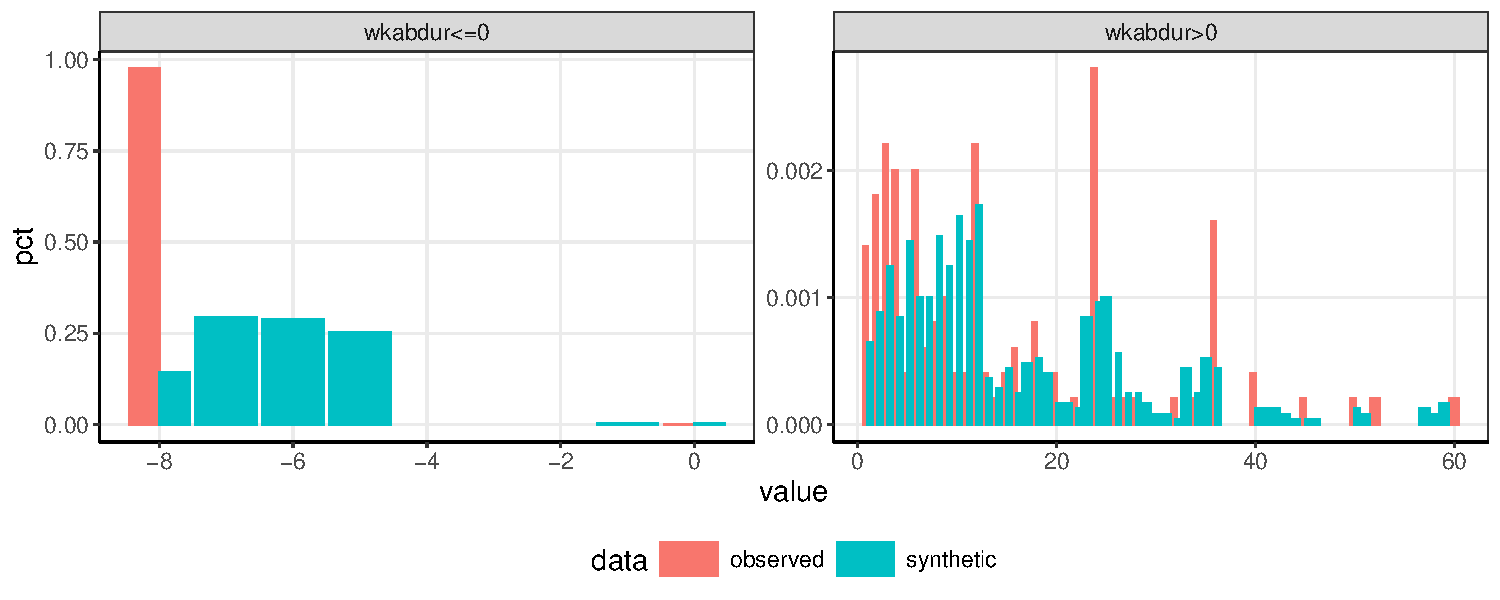
\includegraphics{../graphs/datasynthesizer_wkabdur_1.pdf}}
    \label{fig:ds_variable_wkabdur}
\end{figure}
}

\frame{\frametitle{Solution: Preprocess negative values as missing}
\begin{figure}
    \caption{Work abroad duration - in weeks (wkabdur)}
    \vskip -2mm
    \resizebox{\textwidth}{!}{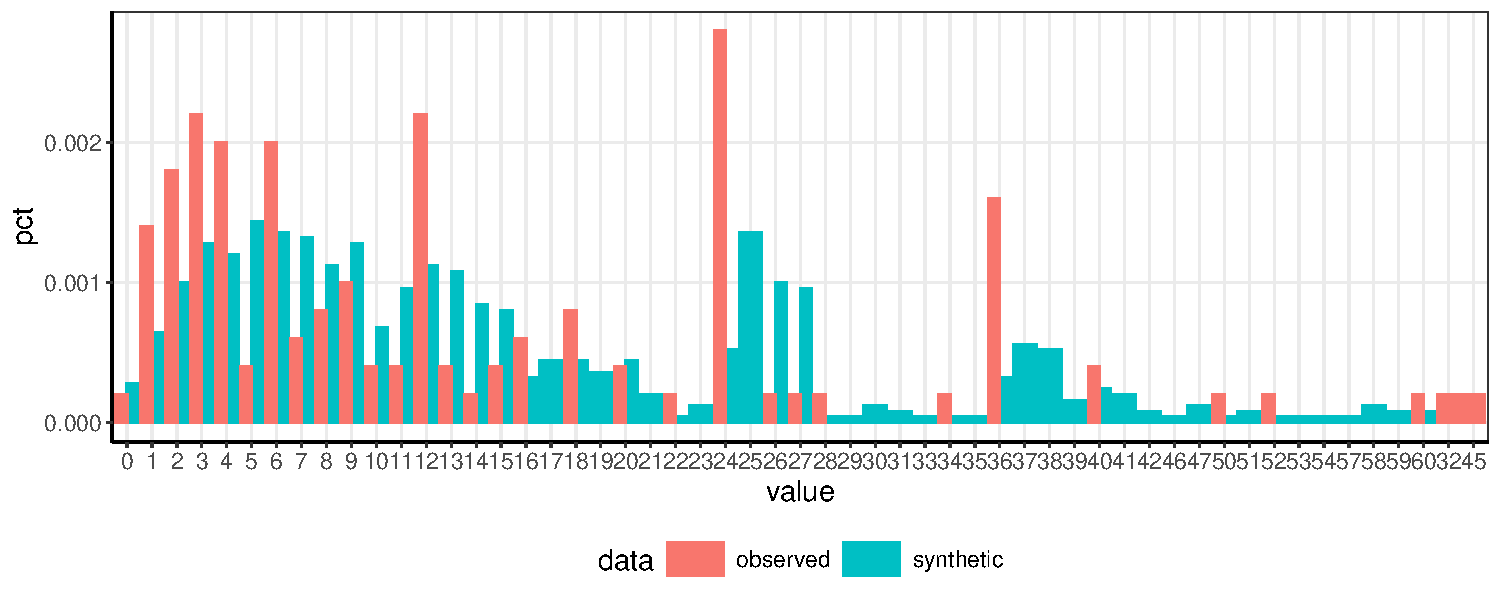
\includegraphics{../graphs/datasynthesizer_wkabdur_clean.pdf}}
    \label{fig:ds_variable_wkabdur_clean}
\end{figure}
}


% \frame{\frametitle{Generated variables (age group)}
% \begin{figure}
%     \caption{Number of misclassified}
%     \vskip -2mm
%     \resizebox{\textwidth}{!}{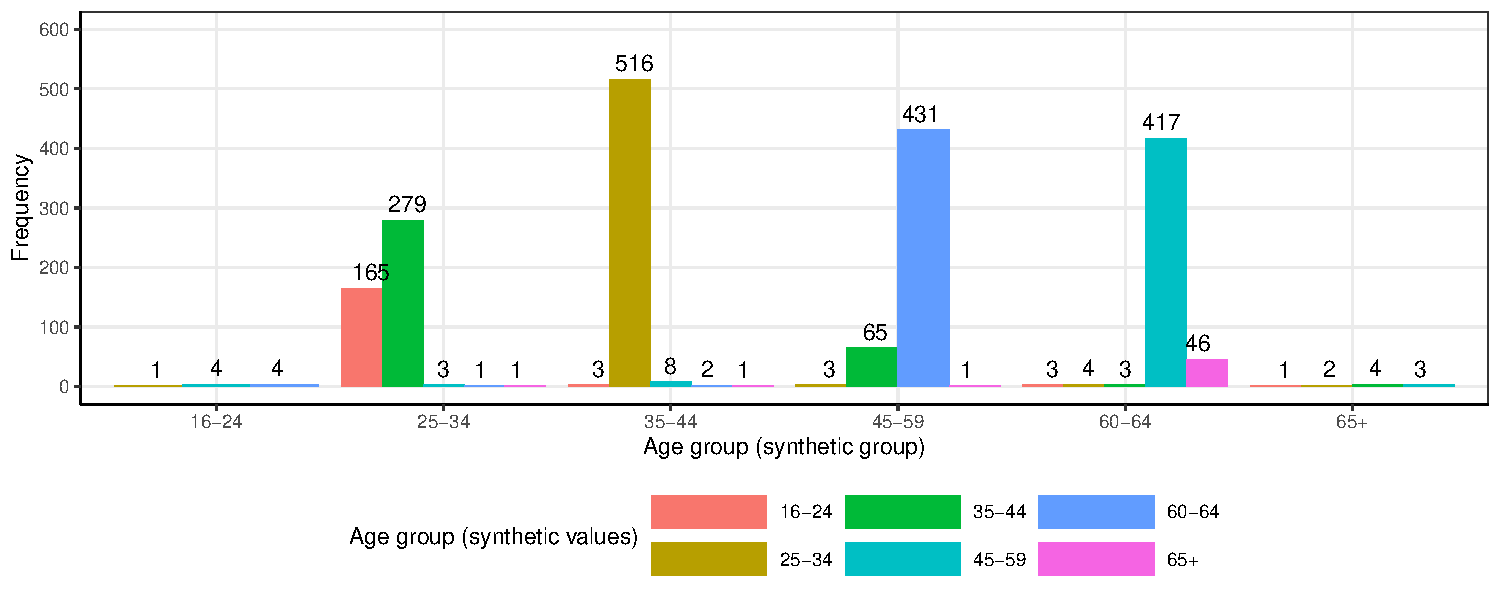
\includegraphics{../graphs/datasynthesizer_frequency_agegr_errors.pdf}}
%     \label{fig:ds_agegr_errors}
% \end{figure}
% }

\frame{\frametitle{Generated variables and extreme values}
\begin{figure}
    \caption{Body mass index (bmi)}
    \vskip -2mm
    \resizebox{\textwidth}{!}{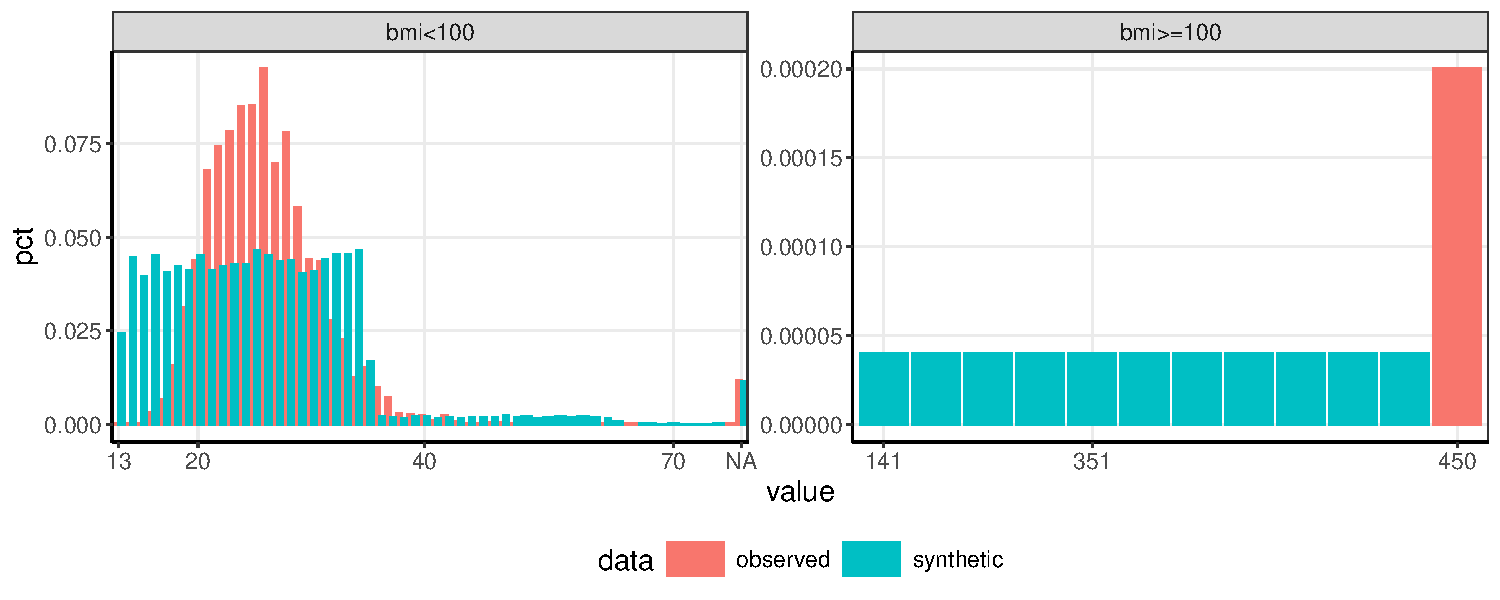
\includegraphics{../graphs/datasynthesizer_bmi.pdf}}
    \label{fig:ds_bmi}
\end{figure}
}

\frame{\frametitle{Solution: Drop generated variables before sending to SDG}
\begin{figure}
    \caption{Regenerate generated values from synthetic values (bmi)}
    \vskip -2mm
    \resizebox{\textwidth}{!}{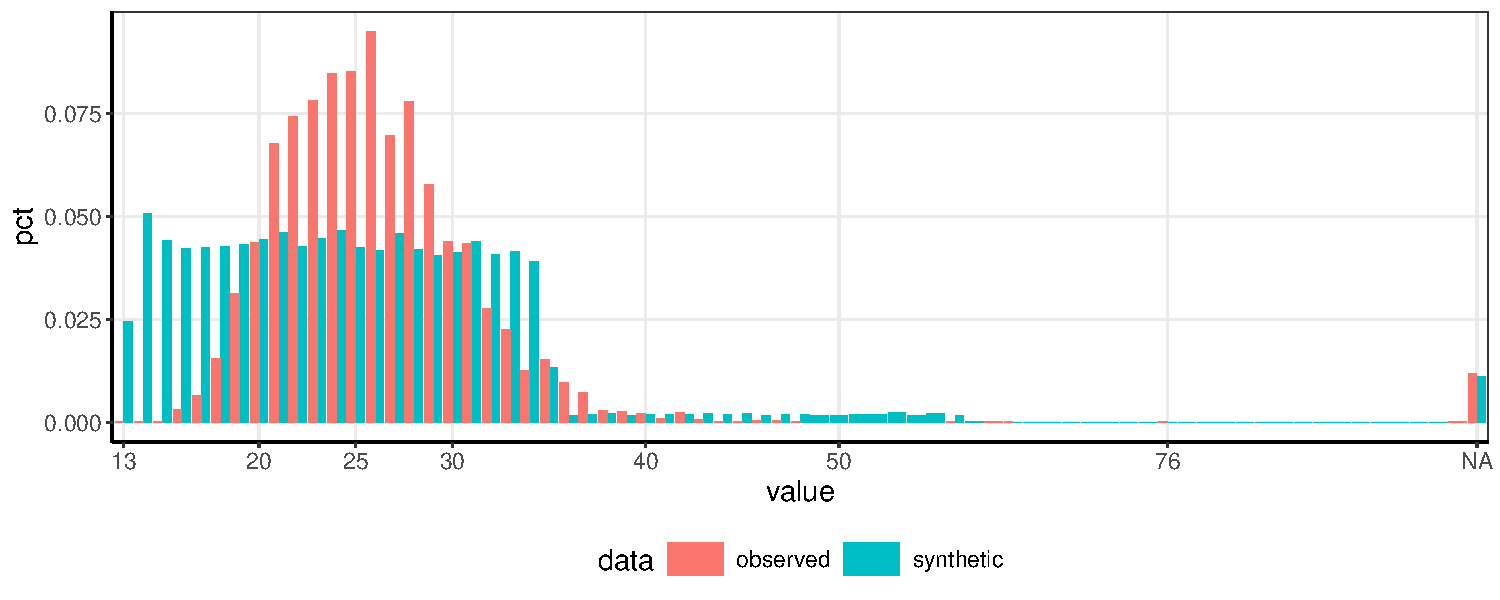
\includegraphics{../graphs/compare_ds_bmi.pdf}}
    \label{fig:compare_ds_bmi.pdf}
\end{figure}
}


% \frame{\frametitle{`Spikey' or discontinuous values}
% \begin{figure}
%     \caption{Number of friends (nofriend)}
%     \vskip -2mm
%     \resizebox{\textwidth}{!}{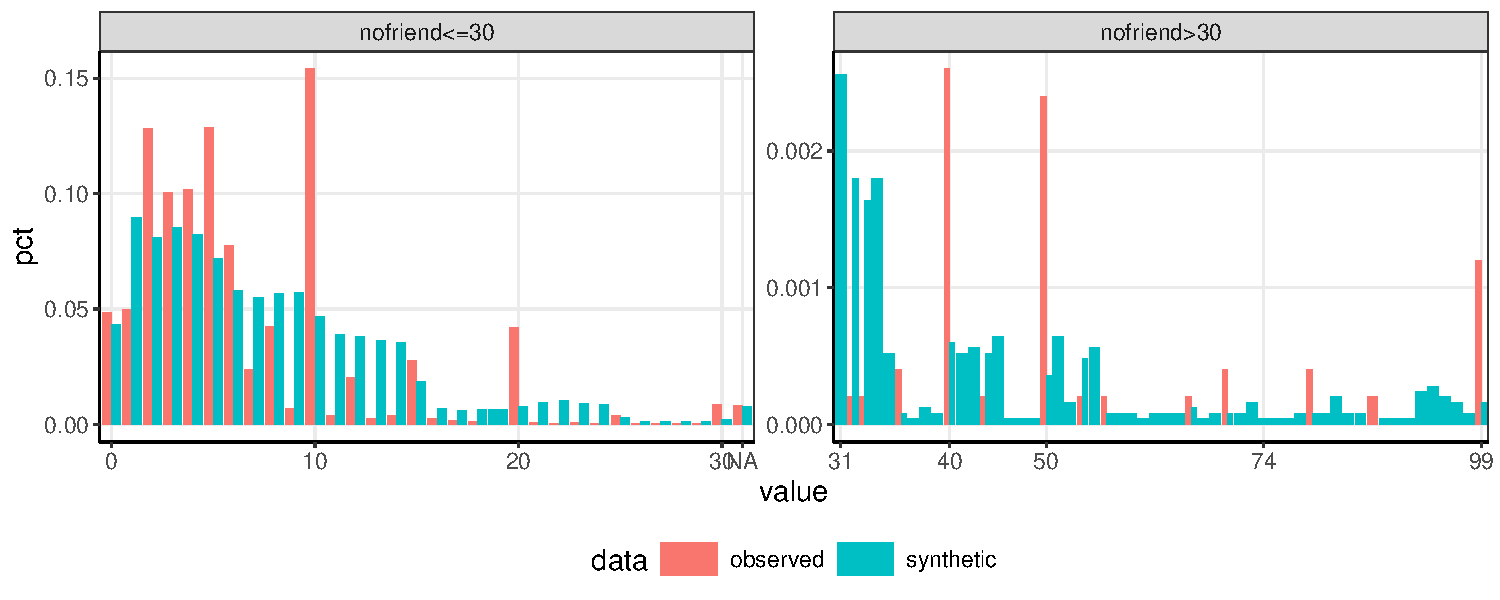
\includegraphics{../graphs/datasynthesizer_nofriend.pdf}}
%     \label{fig:ds_nofriend}
% \end{figure}
% }

\frame{\frametitle{Summary}

\begin{itemize}
    \item The problem: there are consequences of generating random values within a discretized bin
    \item The solution: clean or preprocess the data (code negative values as missing, drop generated variables, etc.)
    \begin{itemize}
        \item But what about `spikey' or discontinuous values?
        \item More generally, cleaning requires knowledge of the data
    \end{itemize}
\end{itemize}
}


% %%%%%%%%%%%%%%
% Sub - section
% %%%%%%%%%%%%%%

\subsection{CTGAN}\label{sec:sdg_ctgan}
\begin{frame}[c,plain]
\vskip-4mm
\begin{beamercolorbox}[wd=\boxwidth,ht=22.11mm]{transparent}%
    \vfill%
    \usebeamerfont{title}%
    \leftinsert%
    \MakeUppercase{Section \ref{sec:sdg}\ref{sec:sdg_ctgan}: Know your generator (CTGAN)} % <- Hier die Überschrift eintragen
\end{beamercolorbox}
\vskip-3mm
\pgfuseimage{rahmenlinie}
\small

\begin{itemize}
    \item Hyperparameters
        \begin{itemize}
            \item Batch size: is the sample size (or rows of data) the GAN looks at at once. (default is 500)
            \item Epochs: Number of times the GAN gets to see the full dataset (default is 300).
            \item Discriminator/Generator dimensions: the number of layers and neurons per layer.  (Default is 2 layers, each with 256 neurons)
            \item Embeddings dimension: the vector size of the compressed representation of the data sent to the generator.  (Default 128)
        \end{itemize}
    \item Utility (pMSE) - similarity or difference between original and synthetic data (lower values are better)
\end{itemize}

% Embedding dimensions indicate the detail of information passed onto the generator, lower is more vague, higher is more detail.

\end{frame}

\frame{\frametitle{Vary batch size}
\begin{figure}
    \caption{DataSynthesizer (0.07) and Synthpop (0.02)}
    \vskip -2mm
    \resizebox{\textwidth}{!}{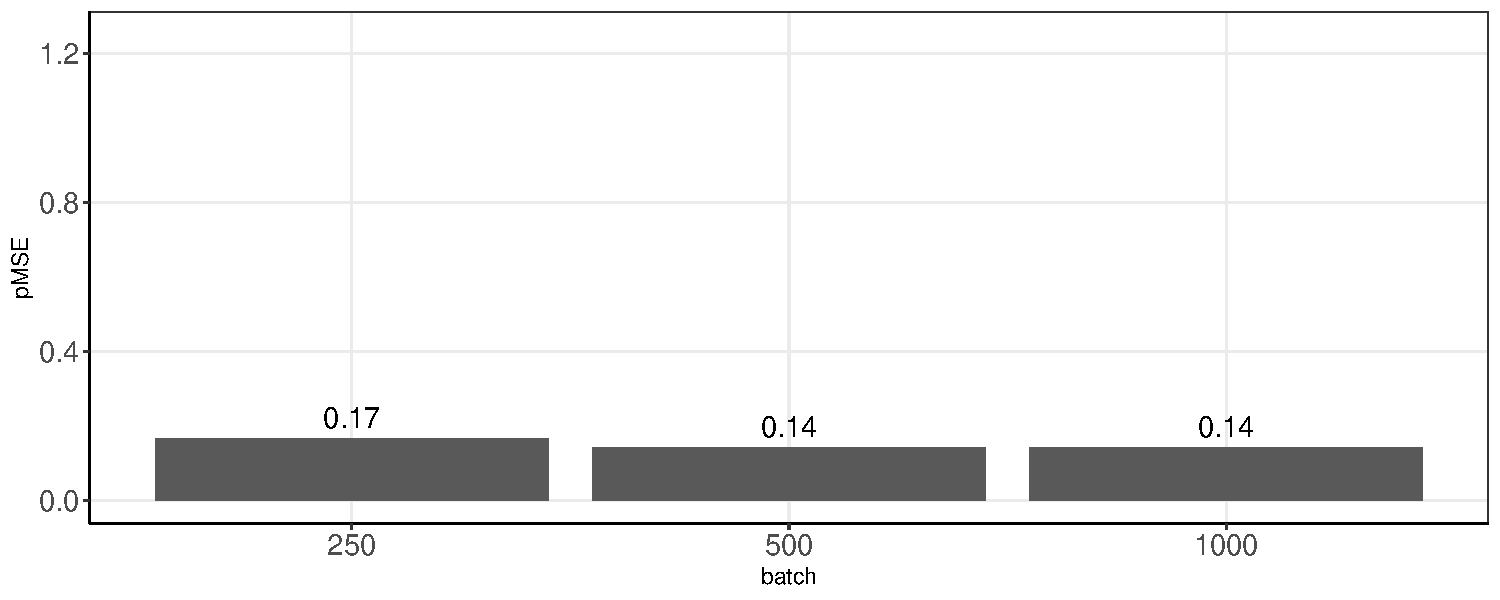
\includegraphics{../graphs/ctgan_fidelity_optimize_batch_size.pdf}}
    \label{fig:ctgan_fidelity_optimize_batch_size.pdf}
\end{figure}
}


\frame{\frametitle{Vary epochs}
\begin{figure}
    \caption{DataSynthesizer (0.07) and Synthpop (0.02)}
    \vskip -2mm
    \resizebox{\textwidth}{!}{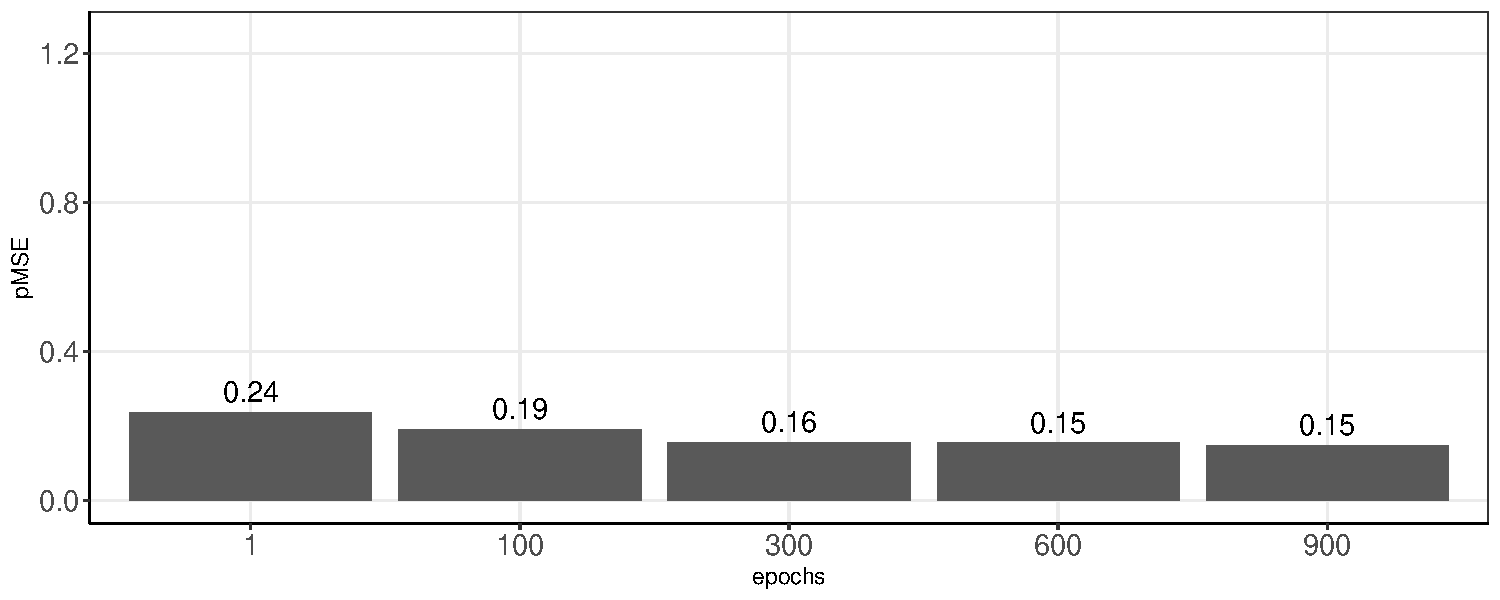
\includegraphics{../graphs/ctgan_fidelity_optimize_epochs.pdf}}
    \label{fig:ctgan_fidelity_optimize_epochs}
\end{figure}
}

\frame{\frametitle{Optimize dimensions}
\begin{figure}
    \caption{DataSynthesizer (0.07) and Synthpop (0.02)}
    \vskip -2mm
    \resizebox{\textwidth}{!}{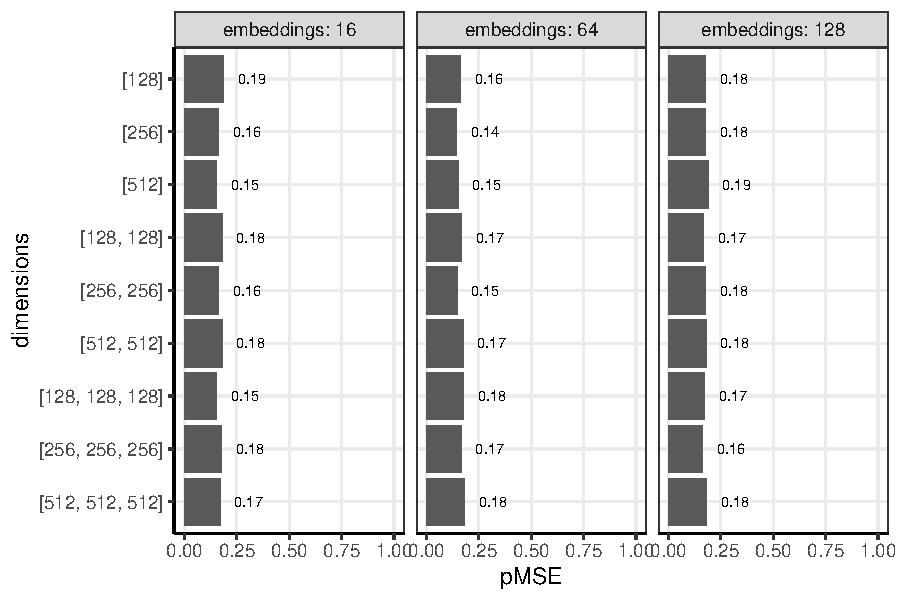
\includegraphics{../graphs/ctgan_fidelity_optimize_dimensions.pdf}}
    \label{fig:ctgan_fidelity_optimize_dimensions}
\end{figure}
}


\frame{\frametitle{Summary}

\begin{itemize}
    \item The problem: CTGAN produces synthetic data with lower utility than DataSynthesizer or Synthpop
    \item Possible explanations 
    \begin{itemize}
        \item GANs are better for high dimensional data (i.e. images).  Our data are low dimensional (33 columns, 5000 rows).
        \item Other GANs might be better.  CTGAN is not the only GAN.  Distinguish between the package and the method.
    \end{itemize}
\end{itemize}
}

% %%%%%%%%%%%%%%
% Sub - section
% %%%%%%%%%%%%%%

\subsection{Synthpop}\label{sec:sdg_synthpop}
\begin{frame}[c,plain]
\vskip-4mm
\begin{beamercolorbox}[wd=\boxwidth,ht=22.11mm]{transparent}%
    \vfill%
    \usebeamerfont{title}%
    \leftinsert%
    \MakeUppercase{Section \ref{sec:sdg}\ref{sec:sdg_synthpop}: Know your generator (Synthpop)} % <- Hier die Überschrift eintragen
\end{beamercolorbox}
\vskip-3mm
\pgfuseimage{rahmenlinie}

\begin{itemize}
    \item Hyperparameters (default)
    \item Utility measure - Computational efficiency
\end{itemize}

\end{frame}

\frame{\frametitle{Computational efficiency}
%eduspec: Discipline of completed qualification
\begin{table}[ht]
    \vskip -2mm
    \caption{}
    \vskip -5mm
    \rowcolors{1}{white}{lightgray}
    \resizebox{\textwidth}{!}{% latex table generated in R 4.4.0 by xtable 1.8-4 package
% Fri Jul 19 16:14:31 2024
\begin{tabular}{llrrrr}
  \toprule
version & description & ctgan & datasynthesizer & synthpop (csv) & synthpop (package) \\ 
  \midrule
v00 & Raw (SD2011) & 331.01 & 245.37 & 2132.12 & 5474.39 \\ 
  v01 & Without eduspec or wkabdur & 290.30 & 264.43 & 10.99 & 8.45 \\ 
  v02 & Without wkabdur & 337.07 & 351.76 & 13.96 & 11.02 \\ 
  v03 & Without eduspec & 306.46 & 351.24 & 11.39 & 8.92 \\ 
  v04 & Last variables: eduspec-wkabdur & 374.57 & 344.02 & 14.23 & 287.85 \\ 
  v05 & Last variables: wkabdur-eduspec & 419.60 & 339.92 & 14.60 & 3657.55 \\ 
  v06 & as.numeric(wkabdur) and last variable: eduspec & 356.02 & 347.36 & 14.12 & 11.05 \\ 
  v07\_1\_20 & + 1 factor variable (20 values) & 339.05 & 264.96 & 42.23 &  \\ 
  v07\_1\_25 & + 1 factor variable (25 values) & 400.28 & 326.84 & 137.47 &  \\ 
  v07\_1\_30 & + 1 factor variable (30 values) & 339.73 & 269.72 & 363.18 &  \\ 
  v07\_2\_20 & + 2 factor variable (20 values) & 369.74 & 339.45 & 74.96 &  \\ 
  v07\_2\_25 & + 2 factor variable (25 values) & 364.56 & 361.81 & 631.43 &  \\ 
  v07\_2\_30 & + 2 factor variable (30 values) & 373.25 & 346.15 & 1222.54 &  \\ 
  v07\_3\_20 & + 3 factor variable (20 values) & 393.99 & 369.58 & 122.77 &  \\ 
  v07\_3\_25 & + 3 factor variable (25 values) & 401.03 & 383.40 & 881.53 &  \\ 
  v07\_3\_30 & + 3 factor variable (30 values) & 394.44 & 424.64 & 3654.59 &  \\ 
   \bottomrule
\end{tabular}
}
    \label{table:table_sd2011_duration_v2}
\end{table}
}

\frame{\frametitle{Summary}

\begin{itemize}
    \item The problem: categorical variables with many values increases the run-time of CART based synthesizers.
    % \item For unordered categorical variables, the number of splits that need to be considered is 2$^{L-1}$ - 1, where L is the number of categories, i.e., the number of splits grows exponentially with the number of categories
    % \item To illustrate, imagine one categorical variable with three values (a, b, and c). There are 3 possible options to split this variable: (1 = a; 0 = b,c), (1 = b; 0 = a,c), (1 = c; 0 = a,b). 
    % \item With six categories, we already need to consider 31 splits, which still doesn't pose a problem computationally. 
    % \item With 20 categories, then 524,288 splits need to be considered
    \item The solution: move categorical variables with many values to the end
    \begin{itemize}
        \item But what about Census data with 3-digit occupation, industry, and country codes?
    \end{itemize}
\end{itemize}
}

% %%%%%%%%%%%%%%
% Section
% %%%%%%%%%%%%%%

\section{Conclusion}\label{sec:conclusion}
\frame{\frametitle{Section \ref{sec:conclusion}: Conclusion}

\begin{itemize}
    \item Contribution: applying SDGs to real data reveal problems not often understood when using clean data 
    \item You need to know your data.    
    \begin{itemize}
        \item Preprocessing or cleaning data is important
        \item This requires knowledge of the data
    \end{itemize}
    \item You need to know your synthesizer 
    \begin{itemize}
        \item DataSynthesizer: Bayesian network model generates random values within discretized bin, but has a hyperparamter for differential privacy 
        \item CTGAN: GAN architecture may not produce synthetic data with high levels of utility, but can synthesize data that others cannot (i.e. images)
        \item Synthpop: CART struggles with computational efficiency on datasets that contain variables with many categories, but produces synthetic data with high utility
    \end{itemize}
    \item The point: 
    \begin{itemize}
        \item You need to match the right synthesizer with the right data problem (no one-size-fits-all solution)
    \end{itemize}
\end{itemize}
}

\frame{\frametitle{Contact}
Jonathan Latner \\
\url{jonathan.latner@iab.de} \\

Reproducible code: 
\begin{itemize}
    \item Github: \url{https://github.com/jonlatner/KEM\_GAN/tree/main/latner/projects/comparison} 
    \item Harvard Dataverse: coming soon
\end{itemize}
}


\end{spacing}
\end{document}

